\documentclass[11pt,a4paper]{article}
\usepackage[utf8]{inputenc}
\usepackage[spanish]{babel}
\usepackage{geometry}
\usepackage{graphicx}
\usepackage{amsmath}
\usepackage{amsfonts}
\usepackage{amssymb}
\usepackage{fancyhdr}
\usepackage{titling}
\usepackage{xcolor}

\geometry{margin=2.5cm}

\definecolor{ubaazul}{RGB}{0,47,95}
\definecolor{ubagris}{RGB}{88,88,90}

\title{SOLUCIONES - PRIMER TRABAJO PRÁCTICO}
\author{Eliana Harriet}
\date{\today}

\begin{document}

\begin{titlepage}
    \centering
    
    \vspace*{0.5cm}
    
    % Logo de la universidad
    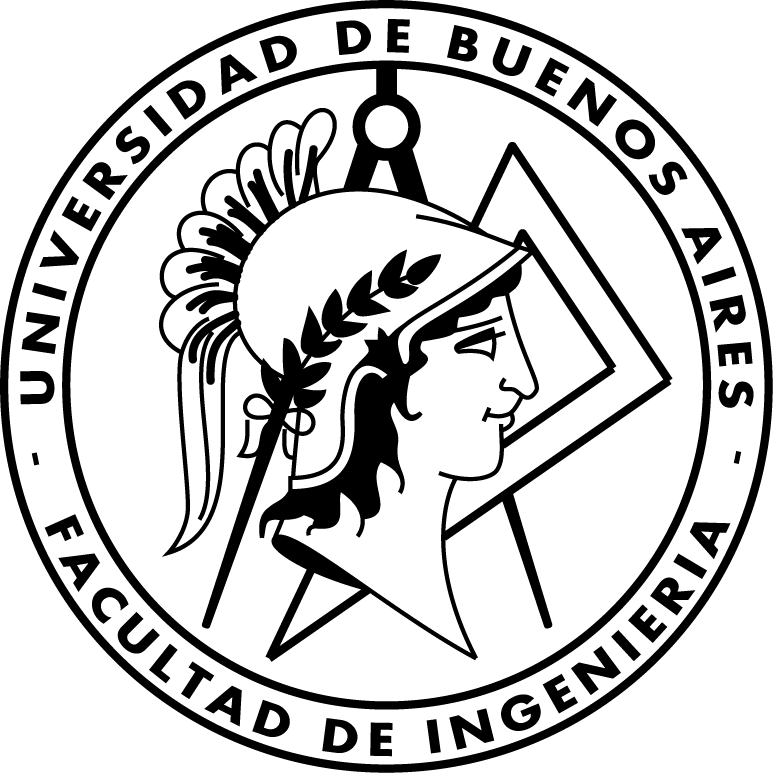
\includegraphics[width=3cm]{../../assets/Logo-fiuba_big.png}\\[0.5cm]
    
    % Encabezado institucional
    {\color{ubaazul}\Large \textbf{UNIVERSIDAD DE BUENOS AIRES}}\\[0.2cm]
    {\color{ubaazul}\large \textbf{Facultad de Ingeniería}}\\[0.1cm]
    {\color{ubagris}\normalsize Laboratorio de Sistemas Embebidos}\\[0.1cm]
    {\color{ubagris}\normalsize Especialización en Inteligencia Artificial}\\[0.3cm]
    
    % Espacio transparente (línea invisible)
    \rule{0cm}{0.5pt}\\[0.5cm]
    
    % Título de la materia
    {\color{ubaazul}\Large \textbf{Probabilidad y Estadística}}\\[0.2cm]
    {\color{ubaazul}\Large \textbf{para la Inteligencia Artificial}}\\[0.8cm]
    
    % Título del documento
    {\Large \textbf{PRIMER TRABAJO PRÁCTICO}}\\[0.5cm]
    
    % Espacio transparente antes de la tabla
    \rule{0cm}{0.5pt}\\[1cm]
    
    % Información en tabla más elegante
    \begin{tabular}{@{}p{4cm}p{7cm}@{}}
        \textbf{Docente:} & Camilo Argoty \\[0.4cm]
        \textbf{Estudiante:} & Eliana Harriet \\[0.4cm]
        \textbf{Código SIU:} & a2217 \\[0.4cm]
        \textbf{Fecha límite:} & 28 de Julio de 2025 \\[0.4cm]
    \end{tabular}
    
    \vfill
    
\end{titlepage}



\tableofcontents
\newpage

\section{Ejercicio 1}
\textbf{Problema de las monedas falsas}

\subsection{Enunciado}
De 10 monedas hay 2 monedas falsas, que tienen probabilidad 0,6 de mostrar cara al ser lanzadas. Si se toma una moneda al azar, se lanza 11 veces, y en todas ellas se obtiene cara, ¿qué es más probable, que la moneda elegida sea justa o que esté cargada? Dar las probabilidades tanto de que la moneda elegida sea falsa, como de que sea justa.

\subsection{Solución}

En el enunciado se menciona la cantidad de monedas totales, 10, de las cuales 2 son falsas y no están balanceadas, 8 sí lo están. De esta forma podemos decir que:

\begin{align*}
P(\text{``Moneda balanceada''}) &= \frac{8}{10} = 0.8 \\
P(\text{``Moneda falsa''}) &= \frac{2}{10} = 0.2
\end{align*}

Una moneda balanceada tendrá la misma probabilidad de que salga cara al tirarla como de que salga seca, por lo tanto $P(\text{``Cara''} | \text{``Moneda balanceada''}) = 0.5$. En el enunciado también se menciona la probabilidad de obtener cara con una moneda falsa, de esta forma podemos decir que $P(\text{``Cara''} | \text{``Moneda falsa''}) = 0.6$.

Ahora, el ejercicio de tomar una moneda con probabilidad $\alpha$ de éxito (obtener cara), tirarla $n$ veces y obtener $k$ éxitos se lo puede modelar con una distribución binomial:

\[
P(X = k) = \binom{n}{k} \alpha^k (1-\alpha)^{n-k}
\]

donde $n$ es el número de lanzamientos, $k$ es el número de éxitos (caras), y $\alpha$ es la probabilidad de éxito en cada lanzamiento.

De esta forma, podemos saber la probabilidad de obtener 11 éxitos en 11 lanzamientos con cada tipo de moneda ($n = k = 11$):

Para una moneda balanceada $\alpha = 0.5$, de esta forma:
\begin{align*}
P(\text{``Cara}^{11}\text{''} | \text{``Moneda balanceada''}) &= \binom{11}{11} (0.5)^{11} (1-0.5)^{11-11} \\
&= 1 \cdot (0.5)^{11} \cdot (0.5)^0 \\
&= (0.5)^{11} = 0.0005
\end{align*}

Para una moneda falsa $\alpha = 0.6$, de esta forma:
\begin{align*}
P(\text{``Cara}^{11}\text{''} | \text{``Moneda falsa''}) &= \binom{11}{11} (0.6)^{11} (1-0.6)^{11-11} \\
&= 1 \cdot (0.6)^{11} \cdot (0.4)^0 \\
&= (0.6)^{11} = 0.0036
\end{align*}

El enunciado pide la probabilidad de que la moneda sea falsa como de que sea una balanceada dado el resultado obtenido. Es decir, hay que obtener $P(\text{``Moneda balanceada''} | \text{``Cara}^{11}\text{''})$ y $P(\text{``Moneda falsa''} | \text{``Cara}^{11}\text{''})$.

Usando el teorema de Bayes para probabilidad condicional:
\[
P(A|B) = \frac{P(B|A) \cdot P(A)}{P(B)}
\]

podemos calcularlas de la siguiente forma:

\begin{align*}
P(\text{``Moneda balanceada''} | \text{``Cara}^{11}\text{''}) &= \frac{P(\text{``Cara}^{11}\text{''} | \text{``Moneda balanceada''}) \cdot P(\text{``Moneda balanceada''})}{P(\text{``Cara}^{11}\text{''})}
\end{align*}

\begin{align*}
P(\text{``Moneda falsa''} | \text{``Cara}^{11}\text{''}) &= \frac{P(\text{``Cara}^{11}\text{''} | \text{``Moneda falsa''}) \cdot P(\text{``Moneda falsa''})}{P(\text{``Cara}^{11}\text{''})}
\end{align*}

Para poder resolver esto es necesario obtener $P(\text{``Cara}^{11}\text{''})$, que puede resolverse usando la ley de probabilidad total como:

\begin{align*}
P(\text{``Cara}^{11}\text{''}) &= P(\text{``Cara}^{11}\text{''} | \text{``Moneda balanceada''}) \cdot P(\text{``Moneda balanceada''}) \\
&\quad + P(\text{``Cara}^{11}\text{''} | \text{``Moneda falsa''}) \cdot P(\text{``Moneda falsa''}) \\
&= 0.0005 \cdot 0.8 + 0.0036 \cdot 0.2 \\
&= 0.0004 + 0.00072 \\
&= 0.00112
\end{align*}

Ahora podemos calcular las probabilidades condicionales que constituyen el objetivo del ejercicio:

\begin{align*}
P(\text{``Moneda balanceada''} | \text{``Cara}^{11}\text{''}) &= \frac{P(\text{``Cara}^{11}\text{''} | \text{``Moneda balanceada''}) \cdot P(\text{``Moneda balanceada''})}{P(\text{``Cara}^{11}\text{''})} \\
&= \frac{0.0005 \cdot 0.8}{0.00112} \\
&= \frac{0.0004}{0.00112} \\
&= 0.357
\end{align*}

\begin{align*}
P(\text{``Moneda falsa''} | \text{``Cara}^{11}\text{''}) &= \frac{P(\text{``Cara}^{11}\text{''} | \text{``Moneda falsa''}) \cdot P(\text{``Moneda falsa''})}{P(\text{``Cara}^{11}\text{''})} \\
&= \frac{0.0036 \cdot 0.2}{0.00112} \\
&= \frac{0.00072}{0.00112} \\
&= 0.643
\end{align*}

Por lo tanto, dado que se obtuvieron 11 caras consecutivas, es más probable que la moneda elegida sea falsa (64.3\%) que balanceada (35.7\%).

\section{Ejercicio 2}
\textbf{Variables aleatorias continuas con densidad conjunta}

\subsection{Enunciado}
Sean $X$ e $Y$ dos v.a. continuas con densidad conjunta:
\[
f_{X,Y} = \begin{cases}
Ky & \text{si } 36x^2 \leq y \leq 9x \\
0 & \text{en otro caso}
\end{cases}
\]

Encontrar:
\begin{enumerate}
    \item[a)] Determine el valor de $K$
    \item[b)] Encuentre la densidad marginal $f_Y(y)$ de $Y$
    \item[c)] Encuentre la densidad condicional $f_{X|Y}(x|y)$ de $X$ dado $Y$
\end{enumerate}

\subsection{Solución}

\textbf{a) Determinación del valor de K}

Para encontrar $K$, usamos la condición de que la integral de la densidad conjunta sobre toda la región debe ser igual a 1.

Primero, determinemos la región de integración. La condición $36x^2 \leq y \leq 9x$ define la región donde la densidad es no nula.

Para que esta región tenga sentido, necesitamos que $36x^2 \leq 9x$, lo cual implica:
\begin{align*}
36x^2 &\leq 9x \\
36x^2 - 9x &\leq 0 \\
9x(4x - 1) &\leq 0
\end{align*}

Esto se cumple cuando $0 \leq x \leq \frac{1}{4}$.

Por lo tanto, la región de integración es: $0 \leq x \leq \frac{1}{4}$ y $36x^2 \leq y \leq 9x$.

\begin{align*}
\int_{-\infty}^{\infty} \int_{-\infty}^{\infty} f_{X,Y}(x,y) \, dx \, dy &= 1 \\
\int_{0}^{1/4} \int_{36x^2}^{9x} Ky \, dy \, dx &= 1
\end{align*}

Resolvemos primero la integral interior con respecto a $y$:
\begin{align*}
\int_{36x^2}^{9x} Ky \, dy &= K \left[ \frac{y^2}{2} \right]_{36x^2}^{9x} \\
&= K \left[ \frac{(9x)^2}{2} - \frac{(36x^2)^2}{2} \right] \\
&= K \left[ \frac{81x^2}{2} - \frac{1296x^4}{2} \right] \\
&= \frac{K}{2} (81x^2 - 1296x^4) \\
&= \frac{81K}{2} x^2 (1 - 16x^2)
\end{align*}

Ahora integramos con respecto a $x$:
\begin{align*}
\int_{0}^{1/4} \frac{81K}{2} x^2 (1 - 16x^2) \, dx &= \frac{81K}{2} \int_{0}^{1/4} (x^2 - 16x^4) \, dx \\
&= \frac{81K}{2} \left[ \frac{x^3}{3} - \frac{16x^5}{5} \right]_{0}^{1/4} \\
&= \frac{81K}{2} \left[ \frac{1}{192} - \frac{1}{320} \right] \\
&= \frac{81K}{2} \left[ \frac{1}{480} \right] \\
&= \frac{27K}{320}
\end{align*}

Por lo tanto:
\begin{align*}
\frac{27K}{320} &= 1 \\
K &= \frac{320}{27}
\end{align*}

\textbf{b) Densidad marginal $f_Y(y)$}

Para encontrar la densidad marginal de $Y$, integramos la densidad conjunta con respecto a $x$:
\[
f_Y(y) = \int_{-\infty}^{\infty} f_{X,Y}(x,y) \, dx
\]

Primero determinamos el rango de $y$. Considerando la región $0 \leq x \leq \frac{1}{4}$ y $36x^2 \leq y \leq 9x$, observamos que $y$ varía desde $0$ (cuando $x = 0$) hasta $\frac{9}{4}$ (cuando $x = \frac{1}{4}$).

Para un valor dado de $y$ en el rango $0 \leq y \leq \frac{9}{4}$, los límites de integración para $x$ se determinan considerando que $x$ debe satisfacer simultáneamente $x \geq \frac{y}{9}$ (proveniente de $y \leq 9x$) y $x \leq \frac{\sqrt{y}}{6}$ (proveniente de $36x^2 \leq y$), es decir, $\frac{y}{9} \leq x \leq \frac{\sqrt{y}}{6}$.

Por lo tanto:
\begin{align*}
f_Y(y) &= \int_{\frac{y}{9}}^{\frac{\sqrt{y}}{6}} \frac{320}{27} y \, dx \\
&= \frac{320y}{27} \left[ x \right]_{\frac{y}{9}}^{\frac{\sqrt{y}}{6}} \\
&= \frac{320y}{27} \left( \frac{\sqrt{y}}{6} - \frac{y}{9} \right) \\
\end{align*}

Simplificando las fracciones:
\begin{align*}
f_Y(y) &= \frac{320y}{27} \left( \frac{\sqrt{y}}{6} - \frac{y}{9} \right)
\end{align*}

Por lo tanto:
\[
f_Y(y) = \begin{cases}
    \frac{320y}{27} \left( \frac{\sqrt{y}}{6} - \frac{y}{9} \right) & \text{si } 0 \leq y \leq \frac{9}{4} \\
0 & \text{en otro caso}
\end{cases}
\]

\textbf{c) Densidad condicional $f_{X|Y}(x|y)$}

La densidad condicional se define como:
\[
f_{X|Y}(x|y) = \frac{f_{X,Y}(x,y)}{f_Y(y)}
\]

Para $0 \leq y \leq \frac{9}{4}$ y $\frac{y}{9} \leq x \leq \frac{\sqrt{y}}{6}$:

\begin{align*}
f_{X|Y}(x|y) &= \frac{\frac{320}{27}y}{\frac{320y}{27} \left( \frac{\sqrt{y}}{6} - \frac{y}{9} \right)} \\
&= \left( \frac{\sqrt{y}}{6} - \frac{y}{9} \right)^{-1}
\end{align*}

Por lo tanto:
\[
f_{X|Y}(x|y) = \begin{cases}
\left( \frac{\sqrt{y}}{6} - \frac{y}{9} \right)^{-1} & \text{si } \frac{y}{9} \leq x \leq \frac{\sqrt{y}}{6} \\
0 & \text{en otro caso}
\end{cases}
\]

\section{Ejercicio 3}
\textbf{Análisis de ventas del supermercado de Don Francisco}

\subsection{Enunciado}
Don Francisco es un pequeño comerciante de barrio que posee un supermercado, con el que sostiene su familia. Uno de sus hijos, Matías, quien recién inicia a cursar la Especialización en Inteligencia Artificial del LSE de la UBA, le propone hacer un análisis de las ventas durante el año anterior, con el fin de hacer pronósticos para el año siguiente, lo que a don Francisco le parece buena idea.

Don Francisco le entrega a Matías el cuaderno donde tiene registrado el valor total de sus ventas en cada día del año. Con esta información, Matías construye una tabla en la cual la primera columna corresponde a la fecha y la segunda corresponde al monto de las ventas, en dólares para evitarse dolores de cabeza con la inflación. Matías no se siente muy seguro de la tarea a realizar, así que les pide ayuda a ustedes para abordar el problema.

A partir del archivo de datos correspondiente a su grupo, determine una función empírica de distribución y una aproximación a la función de densidad de las ventas del supermercado de Don Francisco para cada año de registro (2021, 2022 y 2023).

\subsection{Solución}

\textbf{Datos utilizados}

Se analizaron los datos de ventas diarias del supermercado durante tres años completos (2021, 2022 y 2023), totalizando 1095 observaciones. Los datos están expresados en dólares estadounidenses para evitar complicaciones relacionadas con la inflación.

\textbf{a) Función de densidad}

Para estimar la función de densidad $f(x)$ se utilizó el método de histogramas con la siguiente fórmula:

\[
\hat{f}_h(x) = \frac{1}{nh} \sum_{i=1}^{n} \sum_{j} \mathbf{1}(x_i \in B_j) \mathbf{1}(x \in B_j)
\]

donde:
\begin{itemize}
    \item $\hat{f}_h(x)$ es la función de densidad estimada
    \item $n$ es el número total de observaciones (365 días por año)
    \item $h$ es el ancho del bin (se utilizó $h = 1000$ USD)
    \item $B_j$ representa el $j$-ésimo bin o intervalo del histograma
    \item $\mathbf{1}(\cdot)$ son funciones indicadoras
\end{itemize}

\textbf{Justificación metodológica:} Se seleccionó un ancho de bin de $h = 1000$ USD considerando el rango de datos (aproximadamente \$11,000 - \$28,000 USD) y la necesidad de mantener un equilibrio entre detalle y estabilidad estadística, resultando en aproximadamente 15-17 bins por año.

\textbf{Funciones de densidad estimadas:}

Para cada año se calcularon las siguientes funciones de densidad $\hat{f}_h(x)$ con $h = 1000$ USD:

\textbf{Año 2021:}
\[
\hat{f}_{2021}(x) = \begin{cases}
0.000005 & \text{si } 11631 \leq x < 12631 \\
0.000014 & \text{si } 12631 \leq x < 13631 \\
0.000033 & \text{si } 13631 \leq x < 14631 \\
0.000049 & \text{si } 14631 \leq x < 15631 \\
0.000044 & \text{si } 15631 \leq x < 16631 \\
0.000074 & \text{si } 16631 \leq x < 17631 \\
0.000115 & \text{si } 17631 \leq x < 18631 \\
0.000115 & \text{si } 18631 \leq x < 19631 \\
0.000110 & \text{si } 19631 \leq x < 20631 \\
0.000096 & \text{si } 20631 \leq x < 21631 \\
0.000118 & \text{si } 21631 \leq x < 22631 \\
0.000101 & \text{si } 22631 \leq x < 23631 \\
0.000085 & \text{si } 23631 \leq x < 24631 \\
0.000030 & \text{si } 24631 \leq x < 25631 \\
0.000008 & \text{si } 25631 \leq x < 26631 \\
0.000003 & \text{si } 26631 \leq x < 27631 \\
0 & \text{en otro caso}
\end{cases}
\]

\textbf{Año 2022:}
\[
\hat{f}_{2022}(x) = \begin{cases}
0.000003 & \text{si } 11374 \leq x < 12374 \\
0.000014 & \text{si } 12374 \leq x < 13374 \\
0.000019 & \text{si } 13374 \leq x < 14374 \\
0.000052 & \text{si } 14374 \leq x < 15374 \\
0.000049 & \text{si } 15374 \leq x < 16374 \\
0.000082 & \text{si } 16374 \leq x < 17374 \\
0.000107 & \text{si } 17374 \leq x < 18374 \\
0.000132 & \text{si } 18374 \leq x < 19374 \\
0.000107 & \text{si } 19374 \leq x < 20374 \\
0.000088 & \text{si } 20374 \leq x < 21374 \\
0.000110 & \text{si } 21374 \leq x < 22374 \\
0.000090 & \text{si } 22374 \leq x < 23374 \\
0.000060 & \text{si } 23374 \leq x < 24374 \\
0.000049 & \text{si } 24374 \leq x < 25374 \\
0.000022 & \text{si } 25374 \leq x < 26374 \\
0.000014 & \text{si } 26374 \leq x < 27374 \\
0.000003 & \text{si } 27374 \leq x < 28374 \\
0 & \text{en otro caso}
\end{cases}
\]

\textbf{Año 2023:}
\[
\hat{f}_{2023}(x) = \begin{cases}
0.000005 & \text{si } 11513 \leq x < 12513 \\
0.000008 & \text{si } 12513 \leq x < 13513 \\
0.000016 & \text{si } 13513 \leq x < 14513 \\
0.000041 & \text{si } 14513 \leq x < 15513 \\
0.000077 & \text{si } 15513 \leq x < 16513 \\
0.000085 & \text{si } 16513 \leq x < 17513 \\
0.000074 & \text{si } 17513 \leq x < 18513 \\
0.000110 & \text{si } 18513 \leq x < 19513 \\
0.000134 & \text{si } 19513 \leq x < 20513 \\
0.000093 & \text{si } 20513 \leq x < 21513 \\
0.000164 & \text{si } 21513 \leq x < 22513 \\
0.000099 & \text{si } 22513 \leq x < 23513 \\
0.000041 & \text{si } 23513 \leq x < 24513 \\
0.000025 & \text{si } 24513 \leq x < 25513 \\
0.000016 & \text{si } 25513 \leq x < 26513 \\
0.000008 & \text{si } 26513 \leq x < 27513 \\
0.000000 & \text{si } 27513 \leq x < 28513 \\
0.000003 & \text{si } 28513 \leq x < 29513 \\
0 & \text{en otro caso}
\end{cases}
\]

\textbf{Análisis de las funciones de densidad:}
\begin{itemize}
    \item \textbf{Consistencia}: Las tres funciones muestran formas similares con distribución aproximadamente normal
    \item \textbf{Picos de densidad}: 
    \begin{itemize}
        \item 2021: máximo en \$21,631-\$22,631 ($f = 0.000118$)
        \item 2022: máximo en \$18,374-\$19,374 ($f = 0.000132$)
        \item 2023: máximo en \$21,513-\$22,513 ($f = 0.000164$)
    \end{itemize}
    \item \textbf{Soporte}: Las ventas se concentran entre \$15,000-\$25,000 USD en todos los años
    \item \textbf{Evolución temporal}: 2023 muestra el pico de densidad más alto, sugiriendo mayor concentración de ventas
    \item \textbf{Estabilidad}: La forma de las distribuciones es consistente entre años, indicando un negocio estable
\end{itemize}

\textbf{b) Función de distribución empírica}

La función de distribución empírica se calculó usando:

\[
\hat{F}(x) = \frac{1}{n} \sum_{i=1}^{n} \mathbf{1}(x_i \leq x)
\]

donde $\hat{F}(x)$ estima la probabilidad de que las ventas sean menores o iguales a $x$.

\textbf{Funciones de distribución empírica calculadas:}

Para cada año se calcularon las siguientes funciones de distribución empírica $\hat{F}(x)$:

\textbf{Año 2021:}
\[
\hat{F}_{2021}(x) = \begin{cases}
0.005479 & \text{si } 11631 \leq x < 12631 \\
0.019178 & \text{si } 12631 \leq x < 13631 \\
0.052055 & \text{si } 13631 \leq x < 14631 \\
0.101370 & \text{si } 14631 \leq x < 15631 \\
0.145205 & \text{si } 15631 \leq x < 16631 \\
0.219178 & \text{si } 16631 \leq x < 17631 \\
0.334247 & \text{si } 17631 \leq x < 18631 \\
0.449315 & \text{si } 18631 \leq x < 19631 \\
0.558904 & \text{si } 19631 \leq x < 20631 \\
0.654795 & \text{si } 20631 \leq x < 21631 \\
0.772603 & \text{si } 21631 \leq x < 22631 \\
0.873973 & \text{si } 22631 \leq x < 23631 \\
0.958904 & \text{si } 23631 \leq x < 24631 \\
0.989041 & \text{si } 24631 \leq x < 25631 \\
0.997260 & \text{si } 25631 \leq x < 26631 \\
1.000000 & \text{si } x \geq 26631 \\
0 & \text{si } x < 11631
\end{cases}
\]

\textbf{Año 2022:}
\[
\hat{F}_{2022}(x) = \begin{cases}
0.002740 & \text{si } 11374 \leq x < 12374 \\
0.016438 & \text{si } 12374 \leq x < 13374 \\
0.035616 & \text{si } 13374 \leq x < 14374 \\
0.087671 & \text{si } 14374 \leq x < 15374 \\
0.136986 & \text{si } 15374 \leq x < 16374 \\
0.219178 & \text{si } 16374 \leq x < 17374 \\
0.326027 & \text{si } 17374 \leq x < 18374 \\
0.457534 & \text{si } 18374 \leq x < 19374 \\
0.564384 & \text{si } 19374 \leq x < 20374 \\
0.652055 & \text{si } 20374 \leq x < 21374 \\
0.761644 & \text{si } 21374 \leq x < 22374 \\
0.852055 & \text{si } 22374 \leq x < 23374 \\
0.912329 & \text{si } 23374 \leq x < 24374 \\
0.961644 & \text{si } 24374 \leq x < 25374 \\
0.983562 & \text{si } 25374 \leq x < 26374 \\
0.997260 & \text{si } 26374 \leq x < 27374 \\
1.000000 & \text{si } x \geq 27374 \\
0 & \text{si } x < 11374
\end{cases}
\]

\textbf{Año 2023:}
\[
\hat{F}_{2023}(x) = \begin{cases}
0.005479 & \text{si } 11513 \leq x < 12513 \\
0.013699 & \text{si } 12513 \leq x < 13513 \\
0.030137 & \text{si } 13513 \leq x < 14513 \\
0.071233 & \text{si } 14513 \leq x < 15513 \\
0.147945 & \text{si } 15513 \leq x < 16513 \\
0.232877 & \text{si } 16513 \leq x < 17513 \\
0.306849 & \text{si } 17513 \leq x < 18513 \\
0.416438 & \text{si } 18513 \leq x < 19513 \\
0.550685 & \text{si } 19513 \leq x < 20513 \\
0.643836 & \text{si } 20513 \leq x < 21513 \\
0.808219 & \text{si } 21513 \leq x < 22513 \\
0.906849 & \text{si } 22513 \leq x < 23513 \\
0.947945 & \text{si } 23513 \leq x < 24513 \\
0.972603 & \text{si } 24513 \leq x < 25513 \\
0.989041 & \text{si } 25513 \leq x < 26513 \\
0.997260 & \text{si } 26513 \leq x < 27513 \\
0.997260 & \text{si } 27513 \leq x < 28513 \\
1.000000 & \text{si } x \geq 28513 \\
0 & \text{si } x < 11513
\end{cases}
\]

\textbf{Análisis de las funciones de distribución empírica:}
\begin{itemize}
    \item \textbf{Percentiles clave}:
    \begin{itemize}
        \item $P_{10}$ (10\% de días con ventas menores): $\approx$ \$14,600-\$15,400 USD
        \item $P_{50}$ (mediana): $\approx$ \$19,400-\$20,400 USD  
        \item $P_{90}$ (90\% de días con ventas menores): $\approx$ \$24,400-\$25,400 USD
    \end{itemize}
    \item \textbf{Convergencia}: Las tres funciones alcanzan $F(x) = 1$ entre \$26,600-\$28,500 USD
    \item \textbf{Consistencia temporal}: Distribuciones muy similares entre años, confirmando estabilidad
    \item \textbf{Concentración}: Aproximadamente 80\% de las ventas ocurren en el rango \$15,000-\$25,000 USD
\end{itemize}

\textbf{Conclusiones}

El análisis revela que el supermercado de Don Francisco presenta:
\begin{enumerate}
    \item \textbf{Estabilidad temporal}: Las distribuciones son consistentes entre años
    \item \textbf{Predictibilidad}: El 80\% de los días las ventas están entre \$15,000-\$25,000 USD
    \item \textbf{Distribución normal}: Permite utilizar herramientas estadísticas estándar para pronósticos
    \item \textbf{Baja variabilidad}: La desviación estándar representa aproximadamente 20\% de la media
\end{enumerate}

\textbf{Nota}: El análisis detallado, incluyendo todos los cálculos, gráficos y valores numéricos completos, se encuentra disponible en el notebook Jupyter \texttt{solucion3.ipynb} que se entrega en conjunto.

\end{document}
